\chapter{Figures, tableaux et références}

\section{...}
Chaque figure et chaque tableau doit être référencé. L'ajout des figures et des tableaux à l'aide du \LaTeX\ est simple. Ce chapitre présente quelques exemples de ce processus d'ajout.

\section{Les tableaux}
Le lien suivant explique en détail la manière avec laquelle doit être faite la création et la personnalisation des tableaux à l'aide du \LaTeX\ : \url{https://fr.overleaf.com/learn/latex/Tables}

Le tableau \ref{tab:01} illustre un exemple d'un tableau.

\begin{table}[h]
\centering
\caption{Un exemple d'un tableau.}
\label{tab:01}
\begin{tabular}{|c|c|c|}
\hline
 \textbf{Methods} & \textbf{Result 1} & \textbf{Result 2} \\ 
 \hline
 \textbf{Method 1} & 0.67 & 0.74 \\  
 \hline
 \textbf{Method 2} & 0.86 & 0.90 \\
 \hline
\end{tabular}
\end{table}


\section{Les figures}
Veuillez vous référer au lien suivant pour une description détaillée sur la façon d'insérer des images dans votre document \LaTeX\ et la façon de les référencer dans le texte: \url{https://fr.overleaf.com/learn/latex/Inserting_Images}

La figure \ref{fig:01} illustre une figure qui a été ajoutée juste pour montrer un exemple et la figure \ref{fig:02} illustre une figure principale avec deux sous-figures \ref{fig:02a} and \ref{fig:02b}.

\begin{figure}[h]
\centering
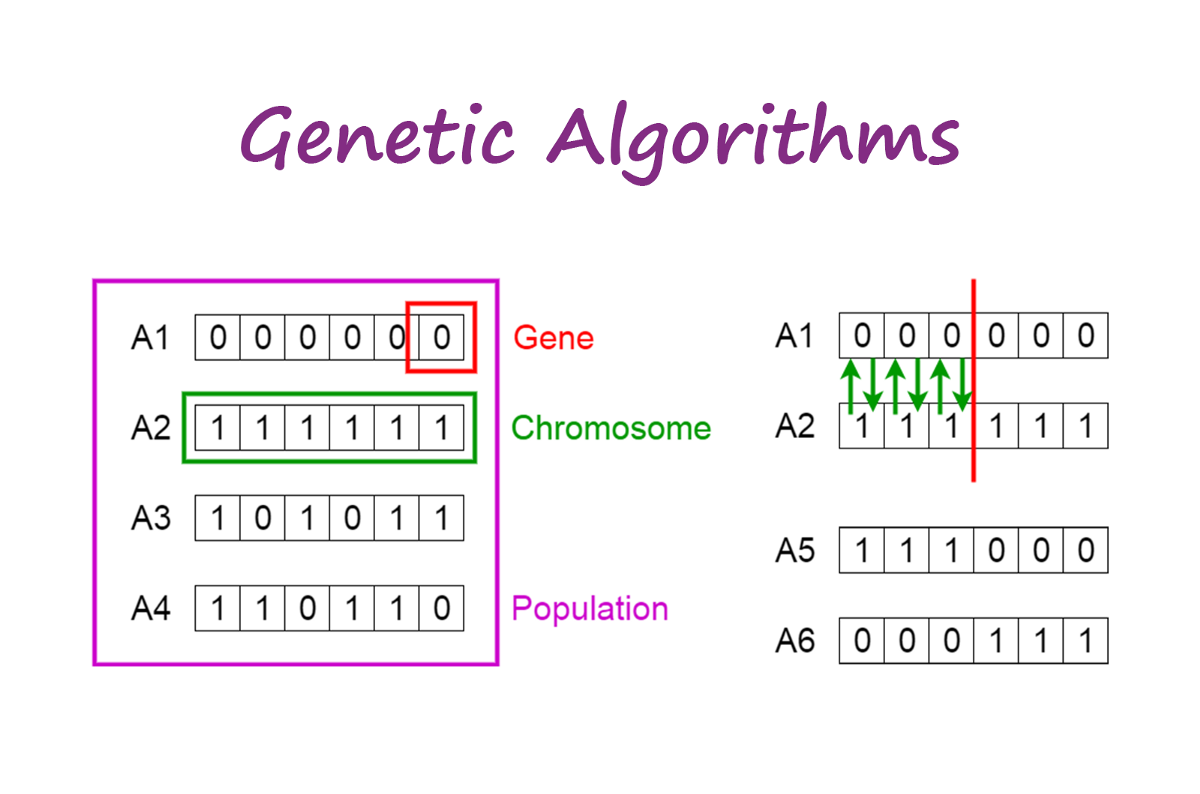
\includegraphics[scale=0.3]{Images/Chapter4/GeneticAlgorithm.png}
\caption{Un exemple d'une figure.}
\label{fig:01}
\end{figure}

~~\\
~~\\



\begin{figure}[h]
     \centering
     \begin{subfigure}[b]{0.4\textwidth}
         \centering
         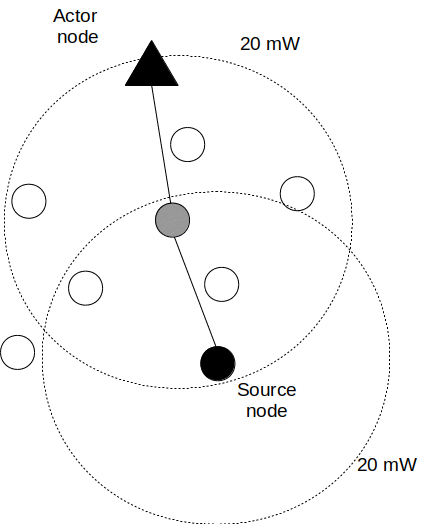
\includegraphics[scale=0.40]{Images/Chapter4/ExempleSansAjustement.png}
         \caption{}
         \label{fig:02a}
     \end{subfigure}
     \hfill
     \begin{subfigure}[b]{0.4\textwidth}
         \centering
         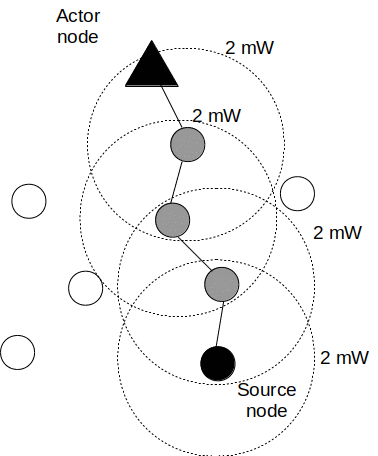
\includegraphics[scale=0.40]{Images/Chapter4/ExempleAvecAjustement.png}
         \caption{}
         \label{fig:02b}
     \end{subfigure}
     \hfill
    \caption{Un exemple d'une figure avec deux sous-figures.}
    \label{fig:02}
\end{figure}

~~\\


\section{Les références}
Les listes de références sont gérées en \LaTeX\ à l'aide de l'outil Bib\TeX\, logiciel de gestion de références bibliographiques développé principalement à cet effet. Voici le lien suivant qui explique en détail comment utiliser Bib\TeX\ :  \url{https://fr.overleaf.com/learn/latex/Bibliography_management_with_bibtex}

Veuillez suivre le style de référence IEEE, pour cela, vous pouvez choisir, par exemple, le style de référence \verb|IEEEtranN|, ce dernier qui nécessite l'invocation du package \verb|natbib| en ajoutant \verb+\usepackage[numbers]{natbib}+ au préambule.

\cite{4}, \cite{2}, \cite{3}, \cite{5}, \cite{1}, ...


\section{...}
\noindent
Acronym of "Intelligence Artificielle": \acrshort{ia} \\
Meaning of MI: \acrlong{mi}
